\documentclass{beamer}
\usepackage{amsmath}
\title{Network Planner:  How it works}
\author{Chris Natali}
\institute{Modi Labs at Columbia University}
\date{October 22, 2012}
\begin{document}

\begin{frame}
  \begin{center}
  {\large Modeling Framework for Network Planning}

  \bigskip

  (Demand Nodes, Parameters) 
  
  $\Downarrow$ 
  
  NP 
  
  $\Downarrow$ 
  
  (Network, Model Outputs)
  \end{center}
\end{frame}

\begin{frame}
  \begin{tabular}{r c l}
    {\tiny Lat, Long, Population, ...} $\rightarrow$ & Demand Nodes & \\
    & $\Downarrow$ & \\
    & Metric Model & $\rightarrow$ {\tiny Projected Population, Demand, Costs} \\
    & $\Downarrow$ & \\
    {\tiny Existing Grid} $\rightarrow$ & Network Model & $\rightarrow$ {\tiny Network} \\
    & $\Downarrow$ & \\
    & Aggregation & $\rightarrow$ {\tiny Totals over all nodes} \\
  \end{tabular}
\end{frame}

\begin{frame}{Electrification Options}
  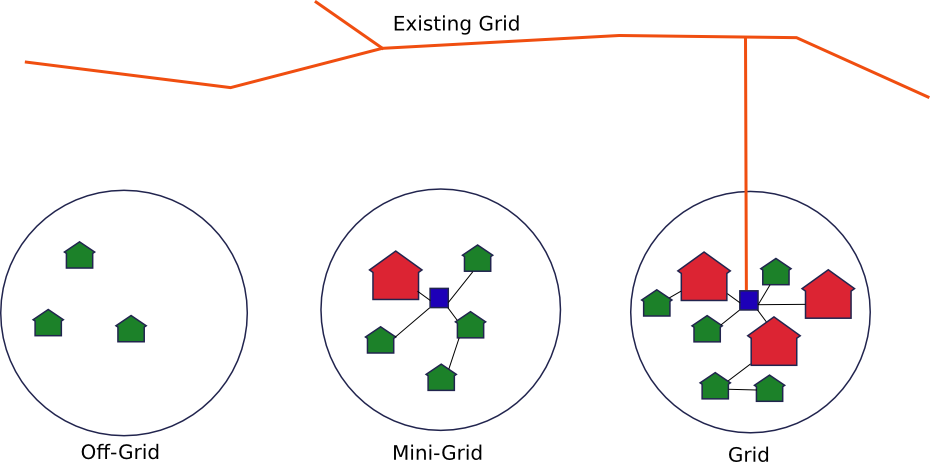
\includegraphics[width=4.0in,height=2.0in]{../diagrams/np-electrification-nodes.png}
\end{frame}


\begin{frame}{Metric Model}
  \begin{tabular}{r c l}
    {\tiny Population, ...} $\rightarrow$ & Demographics &  $\rightarrow$ {\tiny Projected Population, ....} \\
    & $\Downarrow$ & \\
    {\tiny HH Unit Demand per Year, ...} $\rightarrow$ & Demand & $\rightarrow$ {\tiny Projected Demand, ...} \\
    & $\Downarrow$ & \\
        {\tiny Line Cost per Meter, ...} $\rightarrow$ & Costs & $\rightarrow$ {\tiny Projected Grid Internal Cost, ...} \\
    & $\swarrow$ $\searrow$ & \\
    OffGrid Costs & & MiniGrid Costs\\
  \end{tabular}

  \bigskip 

  \begin{center}
  $mvMax = \frac{min(OffGridCost, MiniGridCost) - GridInternalCost}{mvCostPerMeter}$
  \end{center}
\end{frame}

\begin{frame}{Network Model}
  \begin{center}
  Kruskal's MST Algorithm


  Iterate over all candidate segments (node pairs) in ascending length order adding to the network IF they do not create a cycle.

  \bigskip 

  \begin{itemize}
  \item[] Modifications:
  \item[1] Add the condition {\tiny $node1.mvMax \geq segment.length \wedge node2.mvMax \geq segment.length$}
  \item[2] Use ``intersects subnet in more than 1 place" for cycle detection
  \item[3] For segments added and all nodes in their subnet, set {\tiny $mvMax = node1.mvMax + node2.mvMax - segment.length$}
  \end{itemize}
  That last modification ``distributes" demand over the network, increasing it's reach

  \end{center}
\end{frame}
  

\end{document}
